%%%%%%%%%%%%%%%%%%%%%%%%%%%%%%%%%%%%%%%%%
% Short Sectioned Assignment
% LaTeX Template
% Version 1.0 (5/5/12)
%
% This template has been downloaded from:
% http://www.LaTeXTemplates.com
%
% Original author:
% Frits Wenneker (http://www.howtotex.com)
%
% License:
% CC BY-NC-SA 3.0 (http://creativecommons.org/licenses/by-nc-sa/3.0/)
%
%%%%%%%%%%%%%%%%%%%%%%%%%%%%%%%%%%%%%%%%%

%----------------------------------------------------------------------------------------
%	PACKAGES AND OTHER DOCUMENT CONFIGURATIONS
%----------------------------------------------------------------------------------------

\documentclass[paper=b4, fontsize=11pt]{scrartcl} % A4 paper and 11pt font size

\usepackage[T1]{fontenc} % Use 8-bit encoding that has 256 glyphs
\usepackage{fourier} % Use the Adobe Utopia font for the document - comment this line to return to the LaTeX default
\usepackage[english]{babel} % English language/hyphenation
\usepackage{amsmath,amsfonts,amsthm} % Math packages

\usepackage{minted} % Allows to put our code :)
\usepackage{graphicx} % Allows to put images :)
\usepackage[usenames, dvipsnames]{color} % Allows to have color :)
\usepackage{tikz} % Used for drawing state machines
\usepackage{pgf} % Used for drawing state machines
\usetikzlibrary{automata, positioning}
\usetikzlibrary{arrows}

\usepackage{sectsty} % Allows customizing section commands
\allsectionsfont{\centering \normalfont\scshape} % Make all sections centered, the default font and small caps

\usepackage{enumitem}

\usepackage{fancyhdr} % Custom headers and footers
\pagestyle{fancyplain} % Makes all pages in the document conform to the custom headers and footers
\fancyhead{} % No page header - if you want one, create it in the same way as the footers below
\fancyfoot[L]{} % Empty left footer
\fancyfoot[C]{} % Empty center footer
\fancyfoot[R]{\thepage} % Page numbering for right footer
\renewcommand{\headrulewidth}{0pt} % Remove header underlines
\renewcommand{\footrulewidth}{0pt} % Remove footer underlines
\setlength{\headheight}{13.6pt} % Customize the height of the header

\numberwithin{equation}{section} % Number equations within sections (i.e. 1.1, 1.2, 2.1, 2.2 instead of 1, 2, 3, 4)
\numberwithin{figure}{section} % Number figures within sections (i.e. 1.1, 1.2, 2.1, 2.2 instead of 1, 2, 3, 4)
\numberwithin{table}{section} % Number tables within sections (i.e. 1.1, 1.2, 2.1, 2.2 instead of 1, 2, 3, 4)

\setlength\parindent{0pt} % Removes all indentation from paragraphs - comment this line for an assignment with lots of text



%----------------------------------------------------------------------------------------
%	TITLE SECTION
%----------------------------------------------------------------------------------------

\newcommand{\horrule}[1]{\rule{\linewidth}{#1}} % Create horizontal rule command with 1 argument of height
\def\changemargin#1#2{\list{}{\rightmargin#2\leftmargin#1}\item[]}
\let\endchangemargin=\endlist

\title{
\normalfont \normalsize
\textit{In The Name of God} \\ \textsc{Computer Engineering Department of Amirkabir University of Technology} \\ [25pt] \horrule{0.5pt} \\[0.4cm] % Thin top horizontal rule
\huge Design Automation Homework - 5 \\ % The assignment title
\horrule{2pt} \\[0.5cm] % Thick bottom horizontal rule
}

\author{Iman Tabrizian (9331032)}

\date{\normalsize\today}

\begin{document}

\maketitle
\section{Question 6}

\begin{enumerate}[label=(\alph*)]
    \item
        \par Every part of a system has an execution time and every of them
        have a number of exection. Also every of part of the system has subsystems
        and also these parts have hierachy themselves. You can find this statistic
        using \textbf{Profiling} tools.

        \par For codesign we divide the program into two parts. One part is given
        to the software to execute and the other is given to the hardware. This
        act is called \textbf{Partioning}.
    \item
        \par Implementation using software has the benefit of sequential
        execution and also has the benefit of reusing the existing hardware
        components, however hardware implementation has the benefit of
        concurrency and faster execution time but it consumes more resources.
        It is recommended that for the parts that take a lot of time, use the
        hardware implementation while for the parts that don't consume much
        time use the software implementation.
    \item
        \par \textbf{Hard Core} is an actual integrated circuit that does the
        job of central processing unit, while \textbf{Soft Core} is implemented
        in FPGA using the LUTs and there is no actual circuit.

        If we implement a core by ourselves it has the overhead of not being
        optimized. Because both of the above cores are fully optimized. The
        hard core is optimized using electrical elements and the soft core is
        optimized by the vendor that provides it.

    \item
        \begin{enumerate}
            \item
                Point to Point: In this mode the perphial device is directly
                connected to microprocessor. It uses FIFO and transmits data
                in bytestreams.
            \item
                Bus: In this mode there are multiple perphial device on the
                same bus. There is a bus arbiter whose job is to determine the
                periphial device to be connected.
        \end{enumerate}

\end{enumerate}

\section{Question 7}
The circuit that I have found by my self is like below:
\begin{center}
    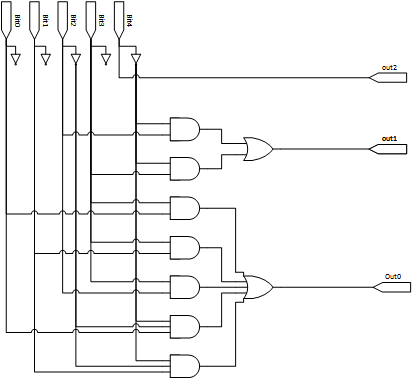
\includegraphics{sqaure_root.png}
\end{center}

In the above circuit the MSB is \textit{bit4} and in the output also
the MSB is \textit{out2}.

\inputminted{vhdl}{q7/src/squareroot.vhd}


And below is the result of delay and area reports:

Memory based method:

+---Adders : \\
	   2 Input     32 Bit       Adders := 1 \\
+---Registers : \\
	               64 Bit    Registers := 3 \\
	               32 Bit    Registers := 1 \\
	                4 Bit    Registers := 1 \\
+---Muxes :                                 \\
	   2 Input     64 Bit        Muxes := 2 \\
	   4 Input     36 Bit        Muxes := 1 \\
	   3 Input      3 Bit        Muxes := 1 \\
	   3 Input      2 Bit        Muxes := 1 \\
	   3 Input      1 Bit        Muxes := 4 \\
	   2 Input      1 Bit        Muxes := 3 \\
	   5 Input      1 Bit        Muxes := 1 \\
Module fsm\\
Detailed RTL Component Info :               \\
+---XORs :                                  \\
	   2 Input      1 Bit         XORs := 1 \\
Module fsm \\
Detailed RTL Component Info :               \\
+---Muxes :                                 \\
	   2 Input      4 Bit        Muxes := 4 \\
Module fsm                       \\
Detailed RTL Component Info :               \\
+---Muxes :                                 \\
	   2 Input      4 Bit        Muxes := 2 \\
	   2 Input      1 Bit        Muxes := 1


The rtl based method:

+---Adders : \\
	   2 Input     32 Bit       Adders := 2 \\
+---Registers : \\
	               64 Bit    Registers := 4 \\
	               32 Bit    Registers := 2 \\
	                4 Bit    Registers := 2 \\
+---Muxes :                                 \\
	   2 Input     64 Bit        Muxes := 3 \\
	   4 Input     36 Bit        Muxes := 2 \\
	   3 Input      3 Bit        Muxes := 2 \\
	   3 Input      2 Bit        Muxes := 2 \\
	   3 Input      1 Bit        Muxes := 5 \\
	   2 Input      1 Bit        Muxes := 4 \\
	   5 Input      1 Bit        Muxes := 2 \\
Module fsm\\
Detailed RTL Component Info :               \\
+---XORs :                                  \\
	   2 Input      1 Bit         XORs := 2 \\
Module fsm \\
Detailed RTL Component Info :               \\
+---Muxes :                                 \\
	   2 Input      4 Bit        Muxes := 5 \\
Module fsm                       \\
Detailed RTL Component Info :               \\
+---Muxes :                                 \\
	   2 Input      4 Bit        Muxes := 3 \\
	   2 Input      1 Bit        Muxes := 2

\section{Question 8}
We should implement this circuit using the memory method:

\begin{tabular}{|c|c|c|c|c|c|c|c|c|}
    \hline
    State bit 2 & State bit 1 & State bit 0 & Input bit 1 & Input bit 0 & Next State bit 2 & Next State bit 1 & Next State bit 0 & Output \\ \hline
    0 & 0 & 0 & 0 & 0 & 0 & 0 & 0 & 0 \\ \hline
    0 & 0 & 0 & 0 & 1 & 0 & 1 & 0 & 0 \\ \hline
    0 & 0 & 0 & 1 & 0 & 1 & 0 & 0 & 0 \\ \hline
    0 & 0 & 0 & 1 & 1 & 0 & 0 & 0 & 0 \\ \hline
    0 & 0 & 1 & 0 & 0 & 0 & 0 & 1 & 1 \\ \hline
    0 & 0 & 1 & 0 & 1 & 0 & 1 & 1 & 1 \\ \hline
    0 & 0 & 1 & 1 & 0 & 1 & 0 & 1 & 1 \\ \hline
    0 & 0 & 1 & 1 & 1 & 0 & 0 & 1 & 1 \\ \hline
    0 & 1 & 0 & 0 & 0 & 0 & 0 & 0 & 0 \\ \hline
    0 & 1 & 0 & 0 & 1 & 0 & 1 & 0 & 0 \\ \hline
    0 & 1 & 0 & 1 & 0 & 1 & 0 & 0 & 0 \\ \hline
    0 & 1 & 0 & 1 & 1 & 0 & 0 & 0 & 0 \\ \hline
    0 & 1 & 1 & 0 & 0 & 0 & 0 & 1 & 1 \\ \hline
    0 & 1 & 1 & 0 & 1 & 0 & 1 & 1 & 1 \\ \hline
    0 & 1 & 1 & 1 & 0 & 0 & 0 & 0 & 0 \\ \hline
    0 & 1 & 1 & 1 & 1 & 0 & 1 & 0 & 0 \\ \hline
    1 & 0 & 0 & 0 & 0 & 1 & 0 & 0 & 0 \\ \hline
    1 & 0 & 0 & 0 & 1 & 0 & 0 & 0 & 0 \\ \hline
    1 & 0 & 0 & 1 & 0 & 0 & 0 & 1 & 1 \\ \hline
    1 & 0 & 0 & 1 & 1 & 0 & 1 & 1 & 1 \\ \hline
    1 & 0 & 1 & 0 & 0 & 1 & 0 & 1 & 1 \\ \hline
    1 & 0 & 1 & 0 & 1 & 0 & 0 & 1 & 1 \\ \hline
    1 & 0 & 1 & 1 & 0 & 0 & 0 & 0 & 0 \\ \hline
    1 & 0 & 1 & 1 & 1 & 0 & 1 & 0 & 0 \\ \hline
\end{tabular}

As you know the default encoding method is sequential and also we have
used sequential encoding explicitly in here.


\inputminted{vhdl}{q8/a/src/fsm.vhd}

And the testbench for this module is like below:


\inputminted{vhdl}{q8/a/test/fsm_tb.vhd}

\section{Question 9}
The source code is like below:


\inputminted{vhdl}{q9/src/arbiter.vhd}

Here is the testbench:

\inputminted{vhdl}{q9/test/arbiter_tb.vhd}


And here is the simulation result:

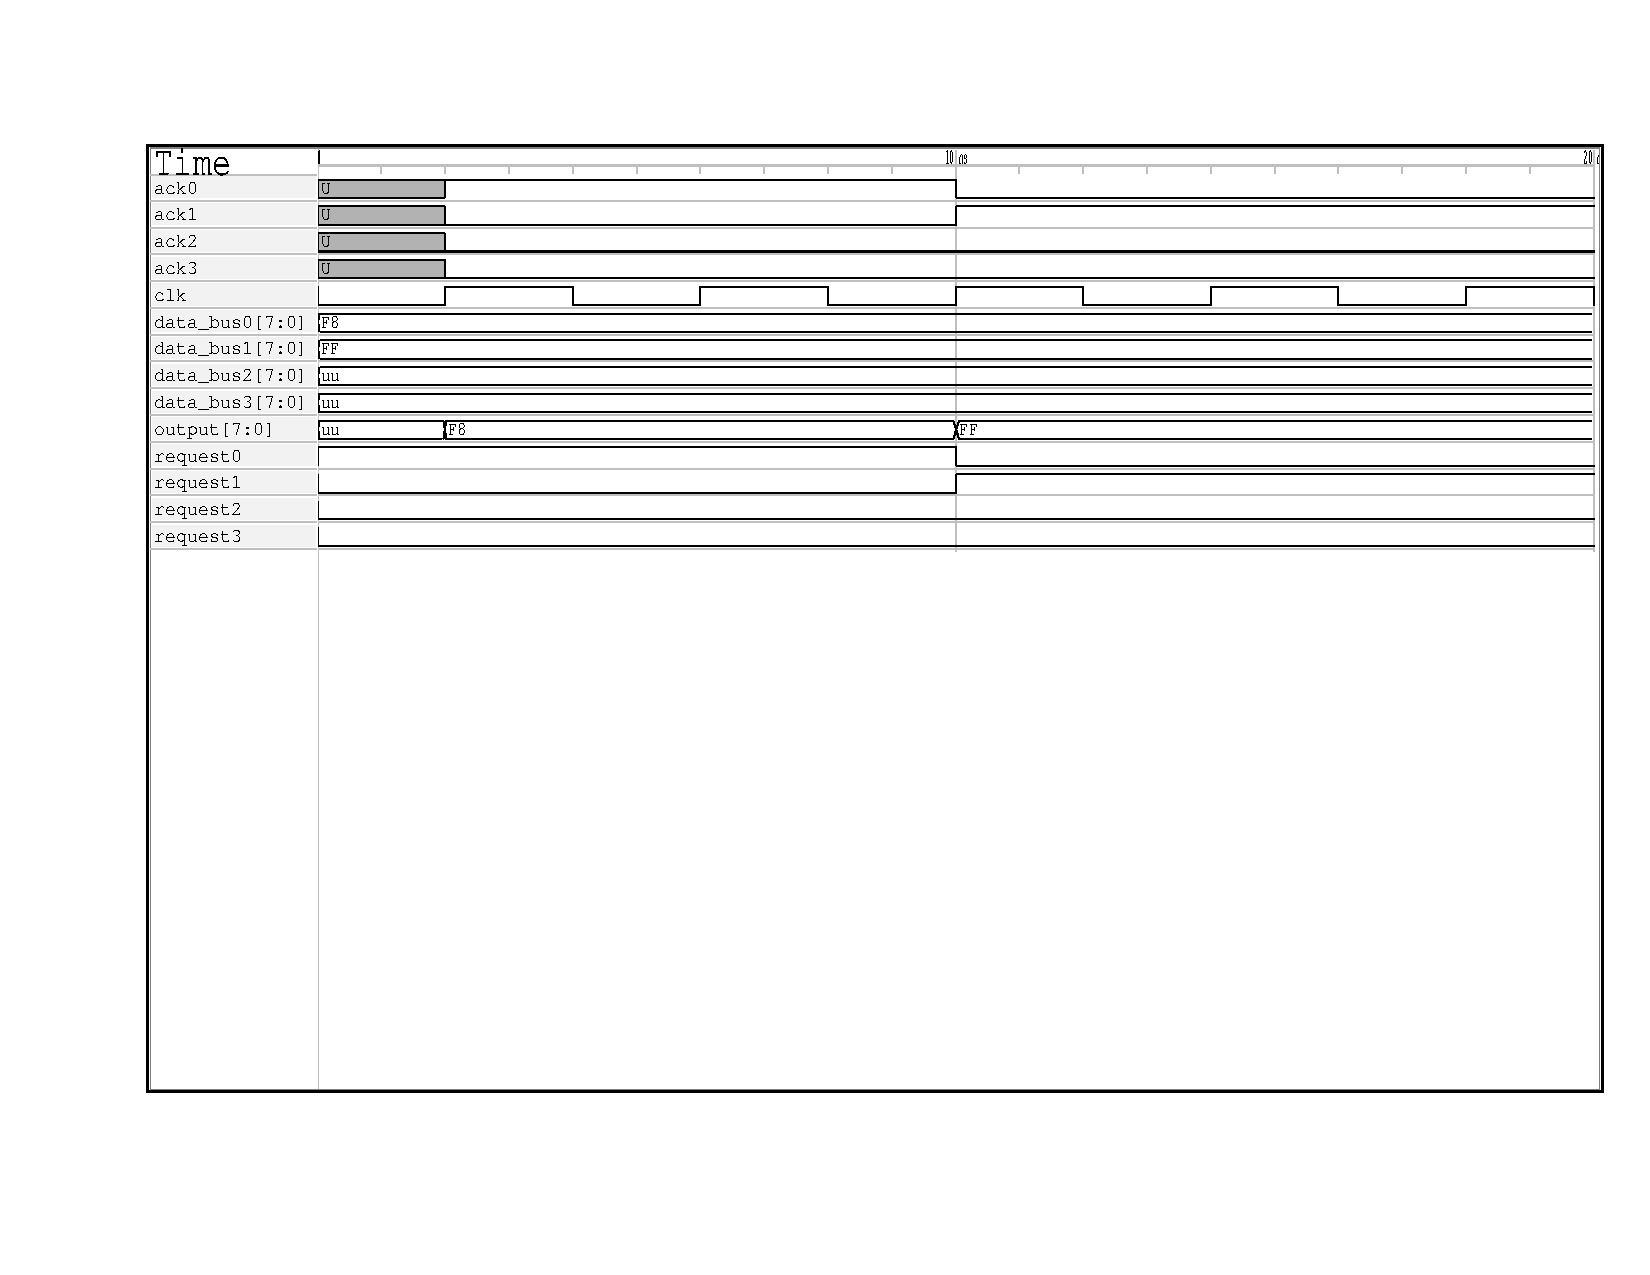
\includegraphics[scale=0.7]{q9/q9_wave.pdf}

\end{document}
